\documentclass[10pt,a4paper]{article}

\usepackage[margin=0.7in]{geometry}
\usepackage[T1]{fontenc}
\usepackage{lmodern}
\usepackage{microtype}
\usepackage{tabularx}
\usepackage{booktabs}
\usepackage{enumitem}
\usepackage{titlesec}
\usepackage[dvipsnames]{xcolor}
\usepackage{tikz}
\usetikzlibrary{arrows.meta,positioning,fit,backgrounds}
\usepackage[hidelinks]{hyperref}

\titleformat{\section}{\large\bfseries}{}{0pt}{}
\titlespacing*{\section}{0pt}{7pt}{3pt}
\setlist{nosep,leftmargin=*}
\setlength{\parskip}{3pt}
\setlength{\parindent}{0pt}

\definecolor{accent}{HTML}{2F6FDB}
\definecolor{edge}{HTML}{8A8A80}
\definecolor{tint}{HTML}{EFEFEC}

\begin{document}

\begin{center}
  {\LARGE\bfseries Exactly-Once GFS: Reliable Record Append\\[2pt] with Raft-Replicated Metadata}\\[6pt]
  {\normalsize Your Name \quad\textbullet\quad Distributed Systems Project Proposal \quad\textbullet\quad 17 October 2026}
\end{center}

\section{Project Description}

This project proposes a GFS-style distributed file system in which record append will be
\textbf{exactly-once for every acknowledged request}, even if the master crashes in the middle of an
append. The original Google File System (SOSP 2003) guarantees only \emph{at-least-once} append: a
retried append can leave duplicate records and padding, and applications must filter them out
themselves. GFS also depends on a single master whose metadata is recovered from an operation log. We
aim to remove both weaknesses, keep data fully replicated when chunk servers fail, and demonstrate the
result by deliberately injecting crashes.

The proposed system will have a \textbf{3-node master group} that replicates all metadata (namespace,
chunk map, leases, and an append-completion table) through \textbf{Raft consensus}, plus \textbf{5 chunk
servers} storing 64\,MB chunks with 3-way replication. Every append will carry a request ID
\texttt{(clientID, seq)} that the client assigns and logs \emph{before} sending. The master will log
each append's intent and its completion as separate Raft entries. That way, a newly elected leader can
always tell which appends were unfinished when the old leader died.

Existing work covers parts of this problem. The MIT 6.5840 labs build Raft with duplicate detection for
key-value stores, and HDFS keeps NameNode metadata highly available with a quorum journal. Neither
combines consensus-backed metadata with deduplicated \emph{record append} across chunk replicas, or
tests every crash point between a metadata update and a chunk update. This project targets that gap.

\begin{figure}[h]
\centering
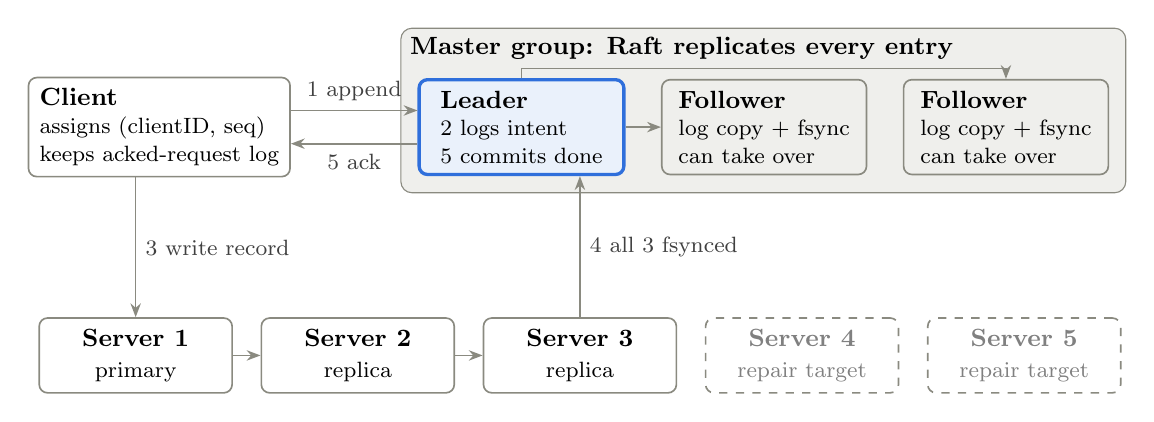
\begin{tikzpicture}[
    font=\small,
    box/.style={draw=edge, rounded corners=3pt, line width=0.6pt, minimum height=1.1cm,
                align=left, inner sep=4pt},
    srv/.style={draw=edge, rounded corners=3pt, line width=0.6pt, minimum width=2.45cm,
                minimum height=0.95cm, align=center},
    idle/.style={srv, dashed, text=gray},
    arr/.style={-{Stealth[length=5pt]}, draw=edge, line width=0.6pt},
    lbl/.style={font=\footnotesize, text=darkgray},
  ]
  % Client
  \node[box, minimum width=3.3cm] (client) at (0,0)
    {\textbf{Client}\\[-1pt]{\footnotesize assigns (clientID, seq)}\\[-1pt]{\footnotesize keeps acked-request log}};

  % Master group
  \node[box, draw=accent, line width=1.2pt, fill=accent!10, minimum width=2.6cm] (leader) at (4.6,0)
    {\textbf{Leader}\\[-1pt]{\footnotesize 2 logs intent}\\[-1pt]{\footnotesize 5 commits done}};
  \node[box, minimum width=2.6cm, right=0.45cm of leader] (f1)
    {\textbf{Follower}\\[-1pt]{\footnotesize log copy + fsync}\\[-1pt]{\footnotesize can take over}};
  \node[box, minimum width=2.6cm, right=0.45cm of f1] (f2)
    {\textbf{Follower}\\[-1pt]{\footnotesize log copy + fsync}\\[-1pt]{\footnotesize can take over}};
  \begin{scope}[on background layer]
    \node[draw=edge, fill=tint, rounded corners=4pt, inner sep=6pt,
          fit=(leader)(f1)(f2), yshift=6pt, inner ysep=12pt] (group) {};
  \end{scope}
  \node[anchor=north west, font=\small\bfseries] at (group.north west) {Master group: Raft replicates every entry};

  % Chunk servers
  \node[srv] (s1) at (-0.3,-2.9) {\textbf{Server 1}\\{\footnotesize primary}};
  \node[srv, right=0.35cm of s1] (s2) {\textbf{Server 2}\\{\footnotesize replica}};
  \node[srv, right=0.35cm of s2] (s3) {\textbf{Server 3}\\{\footnotesize replica}};
  \node[idle, right=0.35cm of s3] (s4) {\textbf{Server 4}\\{\footnotesize repair target}};
  \node[idle, right=0.35cm of s4] (s5) {\textbf{Server 5}\\{\footnotesize repair target}};

  % Arrows
  \draw[arr] ([yshift=6pt]client.east) -- node[lbl, above] {1 append} ([yshift=6pt]leader.west);
  \draw[arr] ([yshift=-6pt]leader.west) -- node[lbl, below] {5 ack} ([yshift=-6pt]client.east);
  \draw[arr] (leader.east) -- (f1.west);
  \draw[arr] (leader.north) -- ++(0,0.12) -| (f2.north);
  \draw[arr] (client.south -| s1.north) -- node[lbl, right] {3 write record} (s1.north);
  \draw[arr] (s1.east) -- (s2.west);
  \draw[arr] (s2.east) -- (s3.west);
  \draw[arr] (s3.north) -- node[lbl, right] {4 all 3 fsynced} (s3.north |- leader.south);
\end{tikzpicture}
\caption{Proposed append path. An append will be acknowledged only after 3 replicas fsync the record
and Raft commits its completion. A master crash between steps 2 and 5 leaves an intent with no
completion, which the new leader settles before serving the client's retry. Each chunk will keep a
request-ID index, and Servers 4--5 will receive new copies when a replica is lost.}
\end{figure}

\section{Goals}

\begin{enumerate}
  \item \textbf{Exactly-once record append.} A retried append with the same request ID must never create
        a second record. The retry will return the original offset if the first attempt committed, or
        run once at a new offset if it was aborted.
  \item \textbf{A precise acknowledgement rule.} The client will receive an ack only when the record is
        fsynced on all 3 chunk replicas \emph{and} its completion entry is committed by a Raft majority
        (2 of 3 masters), so every acked append survives any single master crash.
  \item \textbf{Durable, replicated master metadata.} Namespace, chunk versions, leases and the dedup
        table will live in a Raft log with snapshots and log compaction. The dedup table will be trimmed
        using each client's acknowledged-sequence low-water mark.
  \item \textbf{Fast leader failover.} A new master leader should be elected and serving appends within
        about 2 seconds of a crash (target, to be measured).
  \item \textbf{Recovery of unfinished appends.} After an election, the new leader will find every append
        logged as started but not completed. It will ask the chunk servers which replicas hold that request
        ID, then either commit the append (all replicas have it) or abort it and pad the region so readers
        skip it.
  \item \textbf{Replica health and repair.} The master will track chunk-server heartbeats. When a server
        stops responding, its chunks will be marked \emph{degraded} (2 of 3 replicas), and new appends will
        go to fresh chunks on healthy servers. The master will then copy each degraded chunk, including its
        request-ID index, to a spare server. Chunk version numbers will make sure a returning server's stale
        copies are discarded or brought up to date. Scope: a single failed replica first; a second failure
        during repair if time permits.
  \item \textbf{Live fault-tolerance dashboard.} A web dashboard will show the current leader and Raft term,
        each chunk's replica state (healthy, degraded or repairing), append requests, retries, duplicates
        caught, and recovery and repair progress. It will be fed by an event stream from every node.
  \item \textbf{Crash-point testing with an independent checker.} Crashes will be injected at 5 named points:
        before the intent is logged, after the intent but before any chunk write, after a partial replica
        write, after all replicas write but before completion commits, and after commit but before the
        client hears back. A checker will then compare chunk contents with the client's
        acknowledged-request log.
\end{enumerate}

\section{Tools and Technologies}

{\small
\begin{tabularx}{\textwidth}{@{}l l X@{}}
\toprule
\textbf{Layer} & \textbf{Planned choice} & \textbf{Why} \\
\midrule
Language & Go & Goroutines and channels fit RPC servers and Raft state machines; static binaries are easy to run per node. \\
RPC & gRPC + Protocol Buffers & Typed contracts for client, master and chunk-server calls; streaming for chunk data and repair copies. \\
Consensus & Raft (own, checked vs.\ etcd/raft) & Implementing it ourselves shows the replicated-metadata design; the reference library provides a correctness baseline. \\
Durable storage & WAL + snapshots; checksummed chunk files & Fsync boundaries make every crash point well defined; checksums catch corrupt copies during repair. \\
Deployment & Docker Compose & 3 masters, 5 chunk servers and $N$ clients; one command to start the cluster, kill nodes and restart them. \\
Fault injection & Failpoints, \texttt{docker kill}, \texttt{tc}/\texttt{iptables} & Deterministic crashes between metadata and chunk updates, plus whole-process failures and network partitions. \\
Verification & History checker; Go \texttt{testing} & A Jepsen-style checker and property-based tests compare chunk contents with the acknowledged-request log. \\
Dashboard & Go event stream + WebSocket web UI; Prometheus & The live view of leader, replica health, retries and repair; Prometheus records metrics for the report's charts. \\
\bottomrule
\end{tabularx}
}

\smallskip
{\small Design references: Ghemawat et al., \emph{The Google File System} (SOSP 2003); Ongaro and
Ousterhout, \emph{In Search of an Understandable Consensus Algorithm} (USENIX ATC 2014); the HDFS quorum
journal design.}

\section{Special System Requirements}

Development and the demo will run on one laptop: the 8-node cluster, clients and dashboard fit in Docker
on a 4-core machine with 8--16\,GB RAM and an SSD. No GPU is needed.

The additional resource is for \textbf{large fault-injection campaigns}: thousands of randomized
crash, retry and repair trials. For these we plan to use a few multi-core nodes on the institute's
research compute environment (RCE) to run many isolated clusters in parallel. Durability tests will run
on real disks, never \texttt{tmpfs}, so fsync behaviour is realistic. Open question: how many RCE nodes are
available, and whether Docker is permitted there (if not, nodes will run as plain processes).

\section{Expected Outcomes}

We expect \textbf{zero duplicate or lost acknowledged records} across every crash point and randomized
trial, checked against the client's acknowledged-request log. We also expect every chunk to return to full
3-way replication after a single server failure. The evaluation will report what these guarantees cost.

\textbf{Planned measurements}
\begin{itemize}
  \item Correctness: trials run per crash point, and duplicates or lost acked records found (target: 0).
  \item Failover: time from a master crash to the first successful append on the new leader.
  \item Recovery: time to settle unfinished appends, and how many are committed versus aborted.
  \item Repair: time from losing a replica to full 3-way replication, and append throughput while degraded.
  \item Overhead: append throughput and p50/p99 latency compared with a plain at-least-once GFS baseline built on the same code.
  \item Dedup table size over time, with and without low-water-mark trimming.
\end{itemize}

\textbf{Deliverables}
\begin{enumerate}
  \item Source code: Raft-replicated master, chunk servers with heartbeat-driven repair, client library, and a Docker Compose cluster.
  \item Fault-injection harness with the 5 named crash points, replica-failure scenarios, and a one-command test campaign.
  \item An independent checker that compares stored records with the acknowledged-request log and reports any violation.
  \item The live fault-tolerance dashboard and a demo: kill the leader during an append, watch the retry produce exactly one record, then kill a chunk server and watch its chunks go from degraded to repaired.
  \item A final report with the protocol, invariants, crash-point results and performance charts.
\end{enumerate}

\end{document}
